\documentclass[main]{subfiles}
\begin{document}

\section*{Lecture 12 // Oct 1 // The Chern-Simons Functional \& Reducibles}
\addcontentsline{toc}{section}{Lecture 12 -- The Chern-Simons Functional \& Reducibles}

\textbf{Last time:} We defined the Chern-Simons functional
\[
\CS(A) = \frac{1}{8\pi^2}\int_Y \tr\left(A\wedge dA + \frac{2}{3}A\wedge A\wedge A\right)
\]
and saw that $\grad_A \CS = \ast F_A$. We also interpreted $\Crit(\CS)$ in two ways:
\[
\Crit(\CS) = \{\text{flat connections modulo gauge}\} \leftrightarrow R.
\]

Today, we'll complete the proof of the theorem from last time.

\begin{theorem}
Critical points of the Chern-Simons functional modulo gauge are in bijection with $\SU(2)$ representations of $\pi_1(Y)$ modulo conjugation.
\end{theorem}

\begin{proof}[Proof (continued)]
We must show injectivity. Let $\nabla_0, \nabla_1$ be two connections such that $\hol_p^{\nabla_0}$ and $\hol_p^{\nabla_1}$ are related by conjugation via some fixed $g_p\in \SU(2)$.

We want to show $\nabla_0$ and $\nabla_1$ are gauge equivalent. We construct a global gauge transformation from $g_p$ as follows: for any $q$, choose a path $\gamma$ from $p$ to $q$. Then define
\[
g_q = \hol^{\nabla_1}(\gamma)\circ g_p \circ \hol^{\nabla_0}(\bar\gamma).
\]

\begin{center}
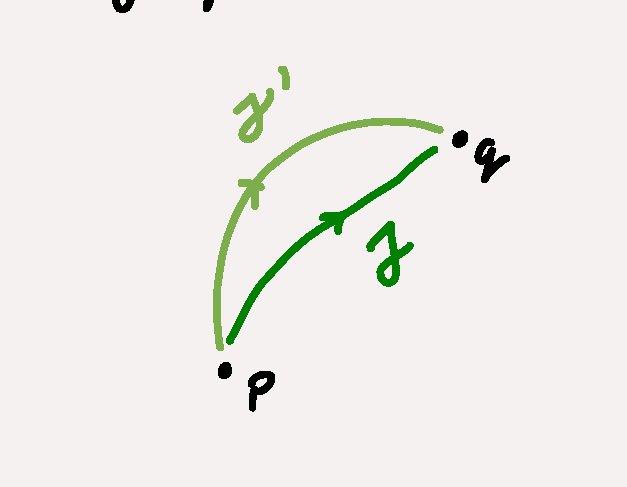
\includegraphics[width=0.3\linewidth]{figures/fig_lec12_path_pq.png}
\end{center}

Is $g_q$ well-defined? Yes: choose another $\gamma'$ from $p$ to $q$. Then $g_q' = \hol^{\nabla_1}(\gamma')\circ g_p\circ \hol^{\nabla_0}(\bar\gamma')$, and
\[
g_q g_q'^{-1} = \left(\hol^{\nabla_1}(\gamma)\circ g_p\circ \hol^{\nabla_0}(\bar\gamma)\right)\circ\left(\hol^{\nabla_1}(\gamma')\circ g_p\circ \hol^{\nabla_0}(\bar\gamma')\right)^{-1}
\]
\[
= \left(\hol^{\nabla_1}(\gamma)\circ g_p\circ \hol^{\nabla_0}(\bar\gamma)\right)\circ \hol^{\nabla_0}(\bar\gamma')^{-1}\circ g_p^{-1}\circ\hol^{\nabla_1}(\gamma')^{-1}
\]
\[
= \hol^{\nabla_1}(\gamma)\circ g_p \circ \hol^{\nabla_0}(\bar\gamma)\circ \hol^{\nabla_0}(\gamma')\circ g_p^{-1}\circ \hol^{\nabla_1}(\bar\gamma').
\]

Since $\hol^{\nabla_0}(\bar\gamma)\circ \hol^{\nabla_0}(\gamma')\in \hol_p^{\nabla_0}$, and $\hol_p^{\nabla_0}$ \& $\hol_p^{\nabla_1}$ are related by $g_p\in \SU(2)$,
\[
g_p\circ \hol^{\nabla_0}(\bar\gamma))\circ \hol^{\nabla_0}(\gamma')\circ g_p^{-1} = \hol^{\nabla_1}(\bar\gamma)\circ \hol^{\nabla_1}(\gamma'),
\]
so
\[
g_qg_q'^{-1} = \hol^{\nabla_1}(\gamma)\circ \hol^{\nabla_1}(\bar\gamma)\circ \hol^{\nabla_1}(\gamma')\circ \hol^{\nabla_1}(\bar\gamma') = \mathrm{id}.
\]

By construction, $\hol^{\nabla_0} = g_q^{-1}\circ \hol^0(\gamma)\cdot g_p$, so certainly the parallel transports of $\nabla_0,\nabla_1$ behave as if related by a gauge transformation. \qedhere
\end{proof}

\subsection*{The Instanton Chain Complex}

Recall that the generators of the Instanton Chain Complex (ICC) are the critical points of the Chern-Simons functional, and the differential is defined by looking at the gradient flow of CS, $\grad_A(\CS) = \ast F_A$. But how can we do this on a three-manifold? The general slogan is that studying the gradient flow of CS on a three-manifold $Y^3$ is the same as studying SD/ASD Yang-Mills connections on $Y^3\times\mathbb{R}$. There's a very precise connection between the three and four-manifold stories; this slogan is the first piece. Specifically, instead of studying (anti)-Self-Dual connections on closed $X^4$, we looked at the open $4$-manifold $\mathbb{R}\times Y$. On $\mathbb{R}\times Y$, consider the trivial $\SU(2)$-bundle $\mathbb{R}\times Y\times \mathbb{C}^2$. By the K\"unneth formula, $c_2(\mathbb{R}\times Y) = \sum_{i+j=2} c_i(\mathbb{R})\otimes c_j(Y) = 0$, so this is only one.

Now let's fix a metric $g_Y$ on $Y$, taking the product metric $dt^2+g_Y$ on $\mathbb{R}\times Y$. We may use this to orient $\mathbb{R}\times Y$ by declaring a positively-oriented basis to be $\{dt,\underbrace{dx,dy,dz}_{Y \text{ directions}}\}$, with $dt$ in the $\mathbb{R}$ direction.

Let's think about the bundle as a $1$-parameter family of objects over $Y$. A gauge transformation $g$ over $\mathbb{R}\times Y$ is a $1$-parameter family of gauge transformations $g_t$: e.g., a gauge transformation on $Y$ smoothly varying with $t$.

A connection (rather, a connection $1$-form) on $\mathbb{R}\times Y$ is, in general, of the form $A = A_t + B_t\, dt$. This is achieved by separating the $dt$ from $dx,dy,dz$ in the $1$-form, so $A_t$ consists of one-forms in $Y$ and $B_t$ is a matrix of $0$-forms. Note that $A_t, B_t$ still vary in $t$, since the $x,y,z$ coordinates are themselves functions of $t$: $x=x(t), y=y(t), z=z(t)$. Also note that $B_t$ is not a connection on $Y$.

For each $t$, define the inclusion map $\iota_t : Y \to \{t\}\times Y \subset \mathbb{R}\times Y$; then $A_t$ is $\iota_t^\ast(A)$. It will be convenient for us to define the following.

\begin{definition}
$A$ is in temporal gauge if $B_t=0$.
\end{definition}

\begin{lemma}
Up to a gauge transformation on $\mathbb{R}\times Y$, every $A$ can be put into temporal gauge.
\end{lemma}

\begin{proof}
We want to find a $1$-parameter family of gauge transformations $\{g_t\}$ which kills the $dt$ component. Applying the transformation law, $g_t$ sends $B_t$ to $g_t^{-1}B_tg_t^{-1} - g_t^{-1}dg_t$. Therefore $g_t$ acts on $A$ via
\[
A \xmapsto{\ \sim g_t\ } g_t^{-1}Ag_t + g_t^{-1}dg_t.
\]
Simplifying,
\[
g_t^{-1}Ag_t + g_t^{-1}dg_t = g_t^{-1}(A_t+B_t\, dt)g_t + g_t^{-1}dg_t = g_t^{-1}A_tg_t + g_t^{-1}B_tg_t\, dt + g_t^{-1}dg_t.
\]

The $dt$ component of $g_t^{-1}dg_t$ is $g_t^{-1}\dfrac{\partial}{\partial t}g_t\, dt$, so the $dt$ component of $g_t^{-1}Ag_t + g_t^{-1}dg_t$ is
\[
g_t^{-1}B_tg_t\, dt + g_t^{-1}\frac{\partial}{\partial t}g_t\, dt.
\]
Therefore we would like to show that for every $t$, there is a $g_t$ such that
\[
g_t^{-1}B_tg_t\, dt + g_t^{-1}\frac{\partial}{\partial t}g_t\, dt = 0.
\]
In other words, we want to solve the $1$-parameter family of ODEs:
\[
g_t^{-1}B_tg_t\, dt + g_t^{-1}\frac{\partial}{\partial t}g_t\, dt = 0 \iff B_tg_t\, dt + \frac{\partial}{\partial t}g_t\, dt = 0 \iff B_tg_t + \frac{\partial}{\partial t}g_t = 0 \iff \frac{\partial}{\partial t}g_t = -B_tg_t.
\]

For each fixed $y\in Y$, we want that $\dfrac{\partial}{\partial t}g_t(y) = -B_t(y)g_t(y)$.

Let's interpret the right hand side. Note that $g_t(y)$ is a path in $\SU(2)$, and $B_t(y)$ is a time-varying element of the Lie algebra of $\SU(2)$, $\mathfrak{su}(2)$, which is the tangent space at the identity $T_{\mathrm{Id}}\SU(2)$. Explicitly, for a fixed $t$ and $y$, $B_t(y)$ is a $2\times 2$ matrix in $\mathfrak{su}(2)$, and $g_t(y)$ is a $2\times 2$ matrix in $\SU(2)$.

We can get a new $2\times 2$ matrix in $\SU(2)$ by right-multiplying $B_t(y)$ by $g_t(y)$:
\[
B_t(y)\cdot g_t(y) = \begin{pmatrix} b_{11}(t,y) & b_{21}(t,y) \\ b_{12}(t,y) & b_{22}(t,y)\end{pmatrix}\cdot \begin{pmatrix} g_{11}(t,y) & g_{21}(t,y) \\ g_{12}(t,y) & g_{22}(t,y)\end{pmatrix}.
\]

\begin{center}
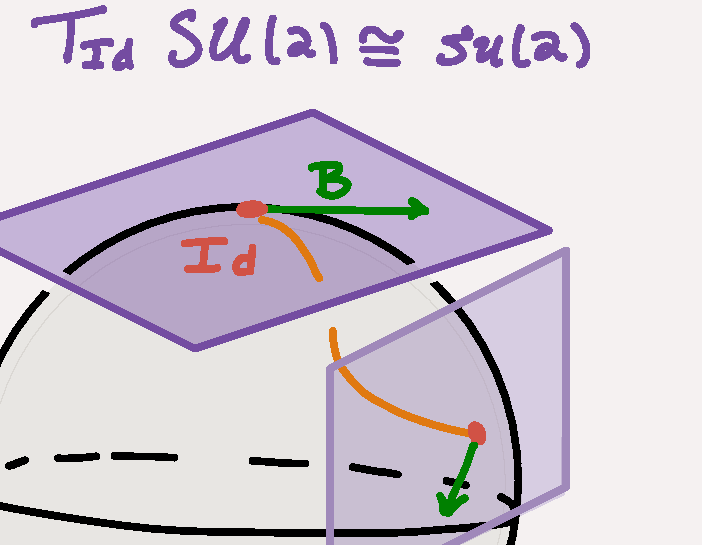
\includegraphics[width=0.3\linewidth]{figures/fig_lec12_tangent_su2.png}
\end{center}

Doing so at each $t$, still fixing $y$, gives us the pushforward of $B_t(y)$ under right multiplication by $g_t(y)$, defining a vector field over all of $\SU(2)$.

Combining this with the left-hand side, if this vector field equals $\dfrac{d}{dt}g_t(y)$, the path must be an integral curve (e.g., a flowline) for this vector field. By ODE theory, this always exists; if the initial conditions are fixed, it is unique. \qedhere
\end{proof}

Up to a gauge transformation, we can think of $\nabla$ on $\mathbb{R}\times Y$ as $\{\nabla_t\}$ on $Y$.

We're now able to ask: what do the SDYM equations look like? First, the self-duality equation is $F_A = \ast F_A$.

Let $A=A_t$ be in temporal gauge. Calculating $F_A = dA + A\wedge A$, note that it's not true that the $4$-dimensional curvature is a $1$-parameter family of $3$-dimensional curvatures. Even though the connection itself has no $dt$ component, the entries of this matrix are functions in all four variables, i.e., these entries are allowed to vary in $t$. This means that $dA$ will have a $\dfrac{\partial}{\partial t}A_t\, dt$ component, which encodes how the curvature of $Y$ changes in the time direction.
\[
dA = dt\wedge \frac{\partial}{\partial t}A_t + \left(\sum_{i=1}^3 dx_i\wedge \frac{\partial}{\partial x_i}A_t\right) = -\frac{\partial}{\partial t}A_t\wedge dt + \underbrace{\left(\sum_{i=1}^3 dx_i\wedge \frac{\partial}{\partial x_i}A_t\right)}_{d^{(3)}A_t}
\]
\[
\Rightarrow F_A = -\frac{\partial}{\partial t}A_t\wedge dt + d^{(3)}A_t + A_t\wedge A_t.
\]

For notational convenience, define $F_{A_t} := d^{(3)}A_t + A_t\wedge A_t$. Then $F_A = -\dfrac{\partial}{\partial t}A_t\wedge dt + F_{A_t}$.

To calculate $\ast F_A$, let's find the relationship between the three and four-dimensional Hodge stars. There are two main cases: if a $2$-form has a time component, and if it doesn't.
\begin{enumerate}
\item $\ast^{(4)}(dx_1\wedge dt) = -dx_2\wedge dx_3 = -\ast^{(3)}dx_1$,
\item $\ast^{(4)}(dx_1\wedge dx_2) = -dx_3\wedge dt = -\ast^{(3)}(dx_1\wedge dx_2)\wedge dt$.
\end{enumerate}

This generalizes to the following relationship: let $i,j,k\in\{1,2,3\}$.
\begin{enumerate}
\item $\ast^{(4)}(dx_i\wedge dt) = -dx_j\wedge dx_k = -\ast^{(3)}dx_i$,
\item $\ast^{(4)}(dx_i\wedge dx_j) = -dx_k\wedge dt = -\ast^{(3)}(dx_i\wedge dx_j)\wedge dt$.
\end{enumerate}

Thus $\ast^{(4)}F_A$ can be expressed using $\ast^{(3)}$ as
\[
\ast^{(4)}F_A = \ast^{(4)}\left(-\frac{\partial}{\partial t}A_t\wedge dt + F_{A_t}\right) = \ast^{(4)}\left(-\frac{\partial}{\partial t}A_t\wedge dt\right) + \ast^{(4)}F_{A_t} = \ast^{(3)}\frac{\partial}{\partial t}A_t - \ast^{(3)}F_{A_t}\wedge dt.
\]

In full, the SDYM equation becomes:
\[
F_A = \ast F_A.
\]
\[
-\frac{\partial}{\partial t}A_t\wedge dt + F_{A_t} = \ast^{(3)}\frac{\partial}{\partial t}A_t - \ast^{(3)}F_{A_t}\wedge dt
\]
\[
\frac{\partial}{\partial t}A_t = \ast^{(3)}F_{A_t}.
\]

For $A=A_t$ in temporal gauge, $A$ is a SD YM connection iff $A_t$ follows $\grad_B\CS = \ast F_B$. Similarly, $A$ is ASD iff $A_t$ is a flow of $-\grad_B\CS$.

Now that we've made sense of what it means to be a generator of the ICC, there's one technical point we must discuss. Just like in the proof of Donaldson's theorem, the space $\mc{A}/\mc{G}$ in the $3$-dimensional setting is not a manifold, since there can be connections with nontrivial stabilizer. Recall that we proved that the stabilizer of a connection is the centralizer of the connection. This holds in the $3$-d case too.

\begin{center}
\begin{tabular}{c|c}
Subgroups of $\SU(2)$ & Centralizer \\
\hline
$I$ & $\SU(2)$ \\
$-I$ & $\SU(2)$ \\
$S^1$ or a conjugate of $S^1$ & $S^1$ \\
Subgroups of $S^1$ or conjugate & $S^1$ \\
non-abelian & $\pm I$ \\
$\SU(2)$ & $\pm I$
\end{tabular}
\end{center}

\begin{lemma}
Flat connections with stabilizer larger than $\pm I$ correspond bijectively to abelian representations of $\pi_1(Y)$, i.e., those which factor through $H_1(Y;\mathbb{Z})$.
\end{lemma}

\begin{definition}
$\nabla$ is called reducible if $\Stab(\nabla)$ is larger than $\pm I$.
\end{definition}

This is the first place we'll use that $Y^3$ is a $\mathbb{Z}\mathrm{HS}^3$. If $Y$ is a homology sphere, there is only one reducible flat connection, which corresponds to the trivial representation into $\SU(2)$.

\begin{remark}
If $Y$ is a $\mathbb{Q}\mathrm{HS}^3$, could have torsion. Computability of $I$ breaks down based on how computable the character variety is, but also on how computable the differential is. The singular points aren't necessarily isolated, but they can be post perturbation.
\end{remark}

\end{document}
